\chapter{Análise de viabilidade}
\minitoc
\label{chap:viabilidad}
\vspace{0.5cm}

%%%%%%%%%%%%%%%%%%%%%%%%%%%%%%%%%%%%%%%%%%%%%%%%%%%%%%%%%%%%%%%%%%%%%%%%%%%%%%%%
% Objetivo: Exponer el análisis de viabilidad del PFC.                         %
%%%%%%%%%%%%%%%%%%%%%%%%%%%%%%%%%%%%%%%%%%%%%%%%%%%%%%%%%%%%%%%%%%%%%%%%%%%%%%%%

\lettrine{N}{este} capítulo exporase a análise de viabilidade do proxecto
baseándose no esquema proporcionado pola planificación inicial: desde o estudo
das solucións xa existentes ata a realización dunha enquisa entre os posibles
usuarios, pasando por un primeiro prototipo.

\section{Planificación inicial}

A continuación (figura \ref{figura:PlanificacionInicialViabilidade}) exponse a
planificación inicial do ciclo de análise da viabilidade.

\begin{figure}[htbp]
 \centering
 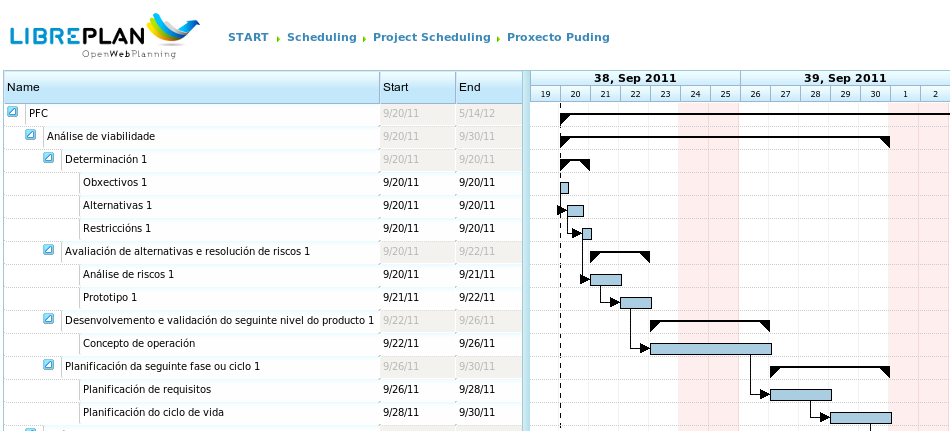
\includegraphics[scale=0.6,keepaspectratio=true]{./imagenes/viabilidade.png}
 % viabilidade.png: 950x431 pixel, 100dpi, 24.13x10.95 cm, bb=0 0 684 310
 \caption{Planificación inicial do ciclo de análise de viabilidade.}
 \label{figura:PlanificacionInicialViabilidade}
\end{figure}

\textbf{Total:} 36 horas.

\section{Determinación}

 \subsection{Obxectivos}

 Establecéronse os obxectivos da fase de análise de viabilidade do proxecto. \\

 Obxectivos:

 \begin{enumerate}
  \item Determinar a viabilidade (1) de deseñar (2) e implementar (3) unha
        gaita MIDI (4) sen fíos (5) en tempo real (6) empregando software (7)/
        hardware (8) libre.
        \footnote{Os números entre parénteses indican a partición do obxectivo
        principal en subobxectivos. Preséntanse así para non distorsionar o
        mesmo. Serán referenciados coma 1.X nas seguintes seccións.}
 \end{enumerate}

 \subsection{Alternativas}

 Establecéronse posibles alternativas a eses obxectivos, aplicables no caso de
 que estes non se puidesen cumprir. \\

 Alternativas:

 \begin{enumerate}
  \item Se non é posible determinar a viabilidade do proxecto, pode optarse
        por:
        \begin{enumerate}
         \item Analizar soamente aquelas partes que sexa posible.
         \item Saltarse completamente a análise de viabilidade e avanzar a
               cegas.
         \item Cancelar e mudar de proxecto
        \end{enumerate}
  \item Se non é posible determinar a viabilidade do deseño, pode optarse por:
        \begin{enumerate}
         \item Analizar soamente aquelas partes do deseño que sexa posible.
         \item Saltarse completamente a análise de viabilidade do deseño e
               avanzar a cegas.
         \item Empregar o deseño dalgunha das solucións xa existentes.
         \item Cancelar e mudar de proxecto.
        \end{enumerate}
  \item Se non é posible determinar a viabilidade da implementación, pode
        optarse por:
        \begin{enumerate}
         \item Analizar soamente aquelas partes da implementación que sexa
               posible.
         \item Saltarse completamente a análise de viabilidade da
               implementación e avanzar a cegas.
         \item Empregar a implementación dalgunha das solucións xa existentes.
         \item Cancelar e mudar de proxecto.
        \end{enumerate}
  \item Se non é posible determinar a viabilidade do emprego do protocolo MIDI,
        pode optarse por:
        \begin{enumerate}
         \item Analizar soamente aquelas partes do protocolo que sexa posible.
         \item Saltarse completamente a análise de viabilidade do protocolo e
               avanzar a cegas.
         \item Empregar outro protocolo similar alternativo.
         \item Cancelar e mudar de proxecto.
        \end{enumerate}
  \item Se non é posible determinar a viabilidade do emprego de tecnoloxía sen
        fíos, pode optarse por:
        \begin{enumerate}
         \item Analizar soamente aquelas partes da tecnoloxía que sexa posible.
         \item Saltarse completamente a análise de viabilidade da tecnoloxía e
               avanzar a cegas.
         \item Empregar conexión por cable.
         \item Cancelar e mudar de proxecto.
        \end{enumerate}
  \item Se non é posible determinar a viabilidade do emprego de tempo real,
        pode optarse por:
        \begin{enumerate}
         \item Analizar soamente aquelas partes nas que sexa posible determinar
               a viabilidade do emprego de tempo real.
         \item Saltarse completamente a análise de viabilidade do emprego de
               tempo real e avanzar a cegas.
         \item Cancelar e mudar de proxecto.
        \end{enumerate}
  \item Se non é posible determinar a viabilidade do emprego de software libre,
        pode optarse por:
        \begin{enumerate}
         \item Analizar soamente aquelas partes nas que sexa posible determinar
               a viabilidade do emprego de software libre.
         \item Saltarse completamente a análise de viabilidade do emprego de
               software libre e avanzar a cegas.
         \item Empregar software privativo nas partes onde non é posible
               determinar a viabilidade do emprego de software libre.
         \item Cancelar e mudar de proxecto.
        \end{enumerate}
  \item Se non é posible determinar a viabilidade do emprego de hardware libre,
        pode optarse por:
        \begin{enumerate}
         \item Analizar soamente aquelas partes nas que sexa posible determinar
               a viabilidade do emprego de hardware libre.
         \item Saltarse completamente a análise de viabilidade do emprego de
               hardware libre e avanzar a cegas.
         \item Empregar hardware privativo nas partes onde non é posible
               determinar a viabilidade do emprego de hardware libre.
         \item Cancelar e mudar de proxecto.
        \end{enumerate}
 \end{enumerate}

 \subsection{Restriccións}

 Establecéronse restriccións aplicables a ditos obxectivos.

 \begin{itemize}
  \item As propias restriccións veñen dadas polo propio título do proxecto. A
        saber:
        \begin{enumerate}
         \item Empregar o protocolo MIDI (1.4).
         \item Empregar tecnoloxía sen fíos (1.5).
         \item Empregar tempo real (1.6).
         \item Empregar software libre (1.7).
         \item Empregar harwdware libre (1.8).
         \item E/ou as derivadas de calquera das súas alternativas.
        \end{enumerate}
 \end{itemize}

\section{Avaliación de alternativas e resolución de riscos}

 \subsection{Análise de riscos}

 Determináronse os riscos que comportaban as distintas alternativas e as súas
 posibles solucións.

 \begin{enumerate}
  \item Alternativas 1.1.
        \begin{enumerate}
         \item Riscos:
               \begin{enumerate}
                \item Que as partes que queden sen analizar sexan inviables.
                \item Que parte ou a totalidade do proxecto sexa inviable.
                \item Que o tempo restante para a execución do proxecto non
                      sexa suficiente.
               \end{enumerate}
         \item Solucións:
               \begin{enumerate}
                \item Aplicar algunha das subsolucións alternativas ou cancelar
                      e mudar de proxecto.
                \item Aplicar algunha das subsolucións alternativas ou cancelar
                      e mudar de proxecto.
                \item Agardar a presentalo na seguinte convocatoria.
               \end{enumerate}
        \end{enumerate}
  \item Alternativas 1.2.
        \begin{enumerate}
         \item Riscos:
               \begin{enumerate}
                \item Que as partes que queden sen analizar sexan inviables.
                \item Que parte ou a totalidade do deseño sexa inviable.
                \item Enxeñería inversa. Alto custe e alta probabilidade de
                      erros no deseño.
                \item Que o tempo restante para a execución do proxecto non
                      sexa suficiente.
               \end{enumerate}
         \item Solucións:
               \begin{enumerate}
                \item Aplicar algunha das subsolucións alternativas ou cancelar
                      e mudar de proxecto.
                \item Aplicar algunha das subsolucións alternativas ou cancelar
                      e mudar de proxecto.
                \item Solicitar o empréstito dos deseños ou cancelar e mudar de
                      proxecto.
                \item Agardar a presentalo na seguinte convocatoria.
               \end{enumerate}
        \end{enumerate}
  \item Alternativas 1.3.
        \begin{enumerate}
         \item Riscos:
               \begin{enumerate}
                \item Que as partes que queden sen analizar sexan inviables.
                \item Que parte ou a totalidade da implementación sexa
                      inviable.
                \item Enxeñería inversa. Alto custe e alta probabilidade de
                      erros na implementación.
                \item Que o tempo restante para a execución do proxecto non
                      sexa suficiente.
               \end{enumerate}
         \item Solucións:
               \begin{enumerate}
                \item Aplicar algunha das subsolucións alternativas ou cancelar
                      e mudar de proxecto.
                \item Aplicar algunha das subsolucións alternativas ou cancelar
                      e mudar de proxecto.
                \item Solicitar o empréstito da implementación ou cancelar e
                      mudar de proxecto.
                \item Agardar a presentalo na seguinte convocatoria.
               \end{enumerate}
        \end{enumerate}
  \item Alternativas 1.4.
        \begin{enumerate}
         \item Riscos:
               \begin{enumerate}
                \item Que as partes que queden sen analizar sexan inviables.
                \item Que parte ou a totalidade do protocolo sexa inviable.
                \item Que non exista protocolo alternativo ou non sexa viable.
                \item Que o tempo restante para a execución do proxecto non
                      sexa suficiente.
               \end{enumerate}
         \item Solucións:
               \begin{enumerate}
                \item Aplicar algunha das subsolucións alternativas ou cancelar
                      e mudar de proxecto.
                \item Aplicar algunha das subsolucións alternativas ou cancelar
                      e mudar de proxecto.
                \item Cancelar e mudar de proxecto.
                \item Agardar a presentalo na seguinte convocatoria.
               \end{enumerate}
        \end{enumerate}
  \item Alternativas 1.5.
        \begin{enumerate}
         \item Riscos:
               \begin{enumerate}
                \item Que as partes que queden sen analizar sexan inviables.
                \item Que parte ou a totalidade da conexión sen fíos sexa
                      inviable.
                \item Que a conexión por cable tampouco sexa viable.
                \item Que o tempo restante para a execución do proxecto non
                      sexa suficiente.
               \end{enumerate}
         \item Solucións:
               \begin{enumerate}
                \item Aplicar algunha das subsolucións alternativas ou cancelar
                      e mudar de proxecto.
                \item Aplicar algunha das subsolucións alternativas ou cancelar
                      e mudar de proxecto.
                \item Cancelar e mudar de proxecto.
                \item Agardar a presentalo na seguinte convocatoria.
               \end{enumerate}
        \end{enumerate}
  \item Alternativas 1.6.
        \begin{enumerate}
         \item Riscos:
               \begin{enumerate}
                \item Que as partes que queden sen analizar sexan inviables.
                \item Que parte ou a totalidade do emprego de tempo real sexa
                      inviable.
                \item Cancelar e mudar de proxecto.
               \end{enumerate}
         \item Solucións:
               \begin{enumerate}
                \item Aplicar algunha das subsolucións alternativas ou cancelar
                      e mudar de proxecto.
                \item Aplicar algunha das subsolucións alternativas ou cancelar
                      e mudar de proxecto.
                \item Agardar a presentalo na seguinte convocatoria.
               \end{enumerate}
        \end{enumerate}
  \item Alternativas 1.7.
        \begin{enumerate}
         \item Riscos:
               \begin{enumerate}
                \item Que as partes que queden sen analizar sexan inviables.
                \item Que parte ou a totalidade do software libre a empregar
                      sexa inviable.
                \item Que non exista software privativo e/ou que o que haxa non
                      sexa viable.
                \item Cancelar e mudar de proxecto.
               \end{enumerate}
         \item Solucións:
               \begin{enumerate}
                \item Aplicar algunha das subsolucións alternativas ou cancelar
                      e mudar de proxecto.
                \item Aplicar algunha das subsolucións alternativas ou cancelar
                      e mudar de proxecto.
                \item Cancelar e mudar de proxecto.
                \item Agardar a presentalo na seguinte convocatoria.
               \end{enumerate}
        \end{enumerate}
  \item Alternativas 1.8.
        \begin{enumerate}
         \item Riscos:
               \begin{enumerate}
                \item Que as partes que queden sen analizar sexan inviables.
                \item Que parte ou a totalidade do hardware libre a empregar
                      sexa inviable.
                \item Que non exista hardware privativo e/ou que o que haxa non
                      sexa viable.
                \item Cancelar e mudar de proxecto.
               \end{enumerate}
         \item Solucións:
               \begin{enumerate}
                \item Aplicar algunha das subsolucións alternativas ou cancelar
                      e mudar de proxecto.
                \item Aplicar algunha das subsolucións alternativas ou cancelar
                      e mudar de proxecto.
                \item Cancelar e mudar de proxecto.
                \item Agardar a presentalo na seguinte convocatoria.
               \end{enumerate}
        \end{enumerate}
 \end{enumerate}

 \subsection{Prototipo 1}

 Realizouse un primeiro prototipo (figura \ref{figura:Prototipo1}) que nos
 permite intuir como será o producto final.

 \begin{figure}[htbp]
  \centering
  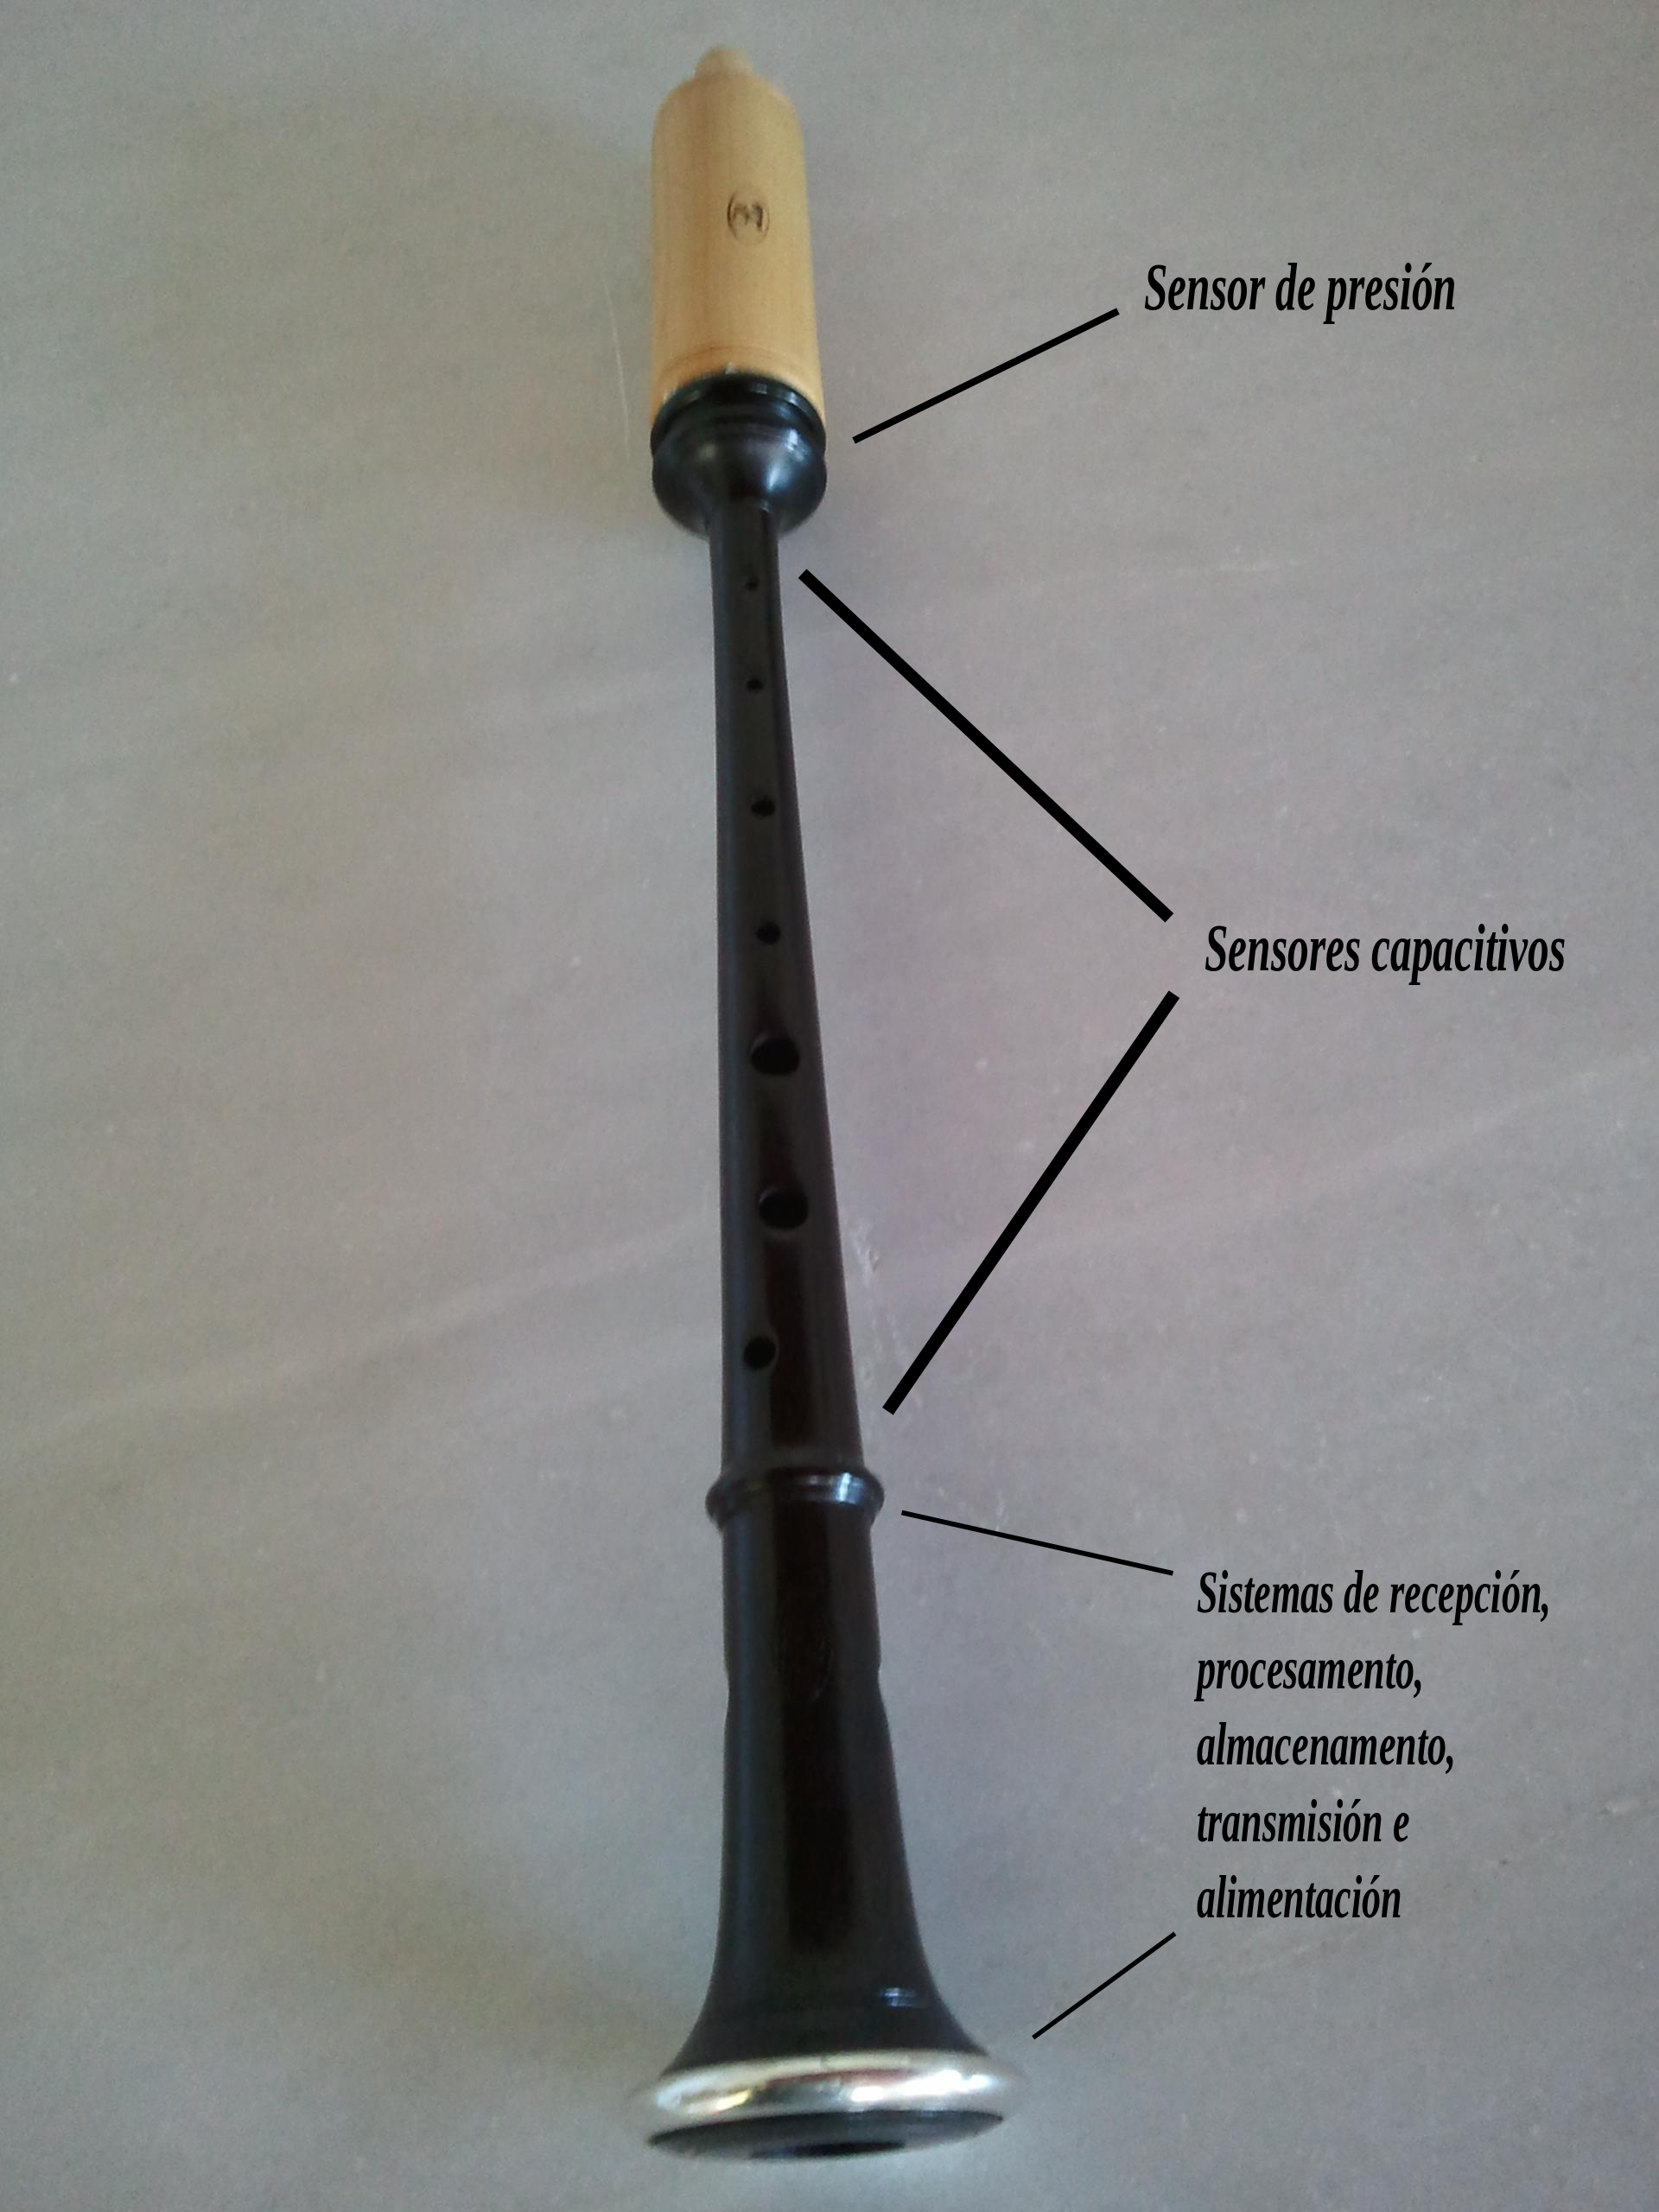
\includegraphics[scale=0.15,keepaspectratio=true]{./imagenes/prototipo1.png}
  % prototipo1.png: 1920x2560 pixel, 72dpi, 67.73x90.31 cm, bb=0 0 1920 2560
  \caption{Prototipo 1.}
  \label{figura:Prototipo1}
 \end{figure}

\section{Desenvolvemento e validación do seguinte nivel do producto}

 \subsection{Concepto de operación}

 Tratouse de definir de maneira conceptual como se operará co producto,
 aclarando que é o que se pretendía conseguir máis exactamente, de xeito que
 fose máis sinxelo obter os requisitos nunha fase posterior. \\

 \begin{figure}[htbp]
  \centering
  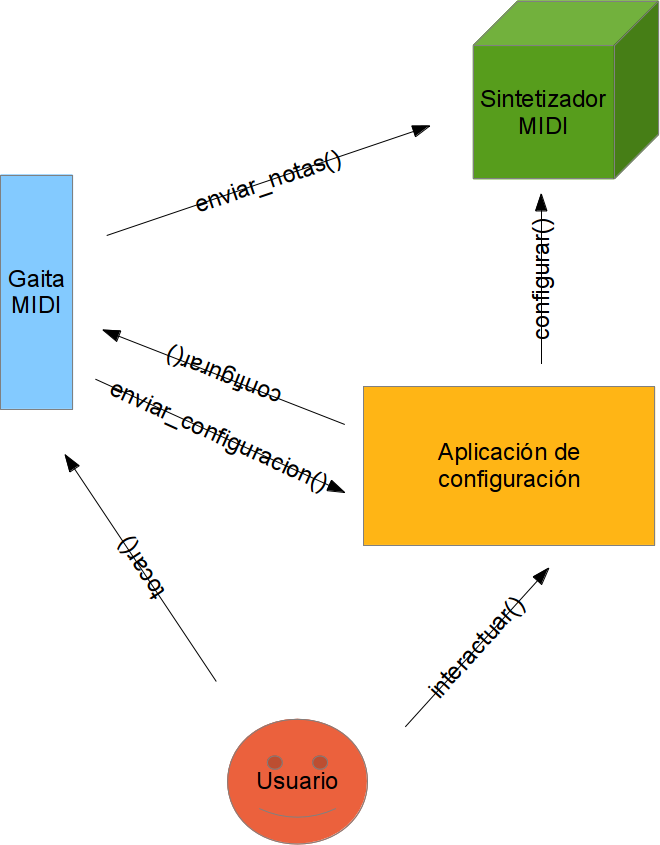
\includegraphics[scale=0.6,keepaspectratio=true]{./imagenes/concepto-operacion.png}
  % concepto-operacion.png: 660x845 pixel, 96dpi, 17.46x22.35 cm, bb=0 0 495 634
  \caption{Concepto de operación.}
  \label{figura:ConceptoOperacion}
 \end{figure}

 Se observamos á gráfica anterior (figura \ref{figura:ConceptoOperacion}) vemos
 que contamos con catro actores:

 \begin{itemize}
  \item \textit{Usuario}: será o encargado de \textit{tocar()} a Gaita MIDI e
        de \textit{interactuar()} coa \textit{Aplicación de configuración}.
  \item \textit{Aplicación de configuración}: será a encargada de
        \textit{configurar()} tanto a \textit{Gaita MIDI} coma o
        \textit{Sintetizador MIDI}.
  \item \textit{Gaita MIDI}: será a encargada de \textit{enviar\_notas()} ó
        \textit{Sintetizador MIDI} e de \textit{enviar\_configuracion()} á
        \textit{Aplicación de configuración}.
  \item \textit{Sintetizador MIDI}: será o encargado de \textit{reproducir()} as
        notas ou mensaxes MIDI que lle chegan da \textit{Gaita MIDI}.
 \end{itemize}

\section{Planificación da seguinte fase ou ciclo}

 \subsection{Planificación de requisitos}

 A continuación (figura \ref{figura:PlanificacionInicialRequisitos}) exponse a
 planificación inicial do ciclo de análise de requisitos. \\

 \begin{figure}[htbp]
 \centering
 %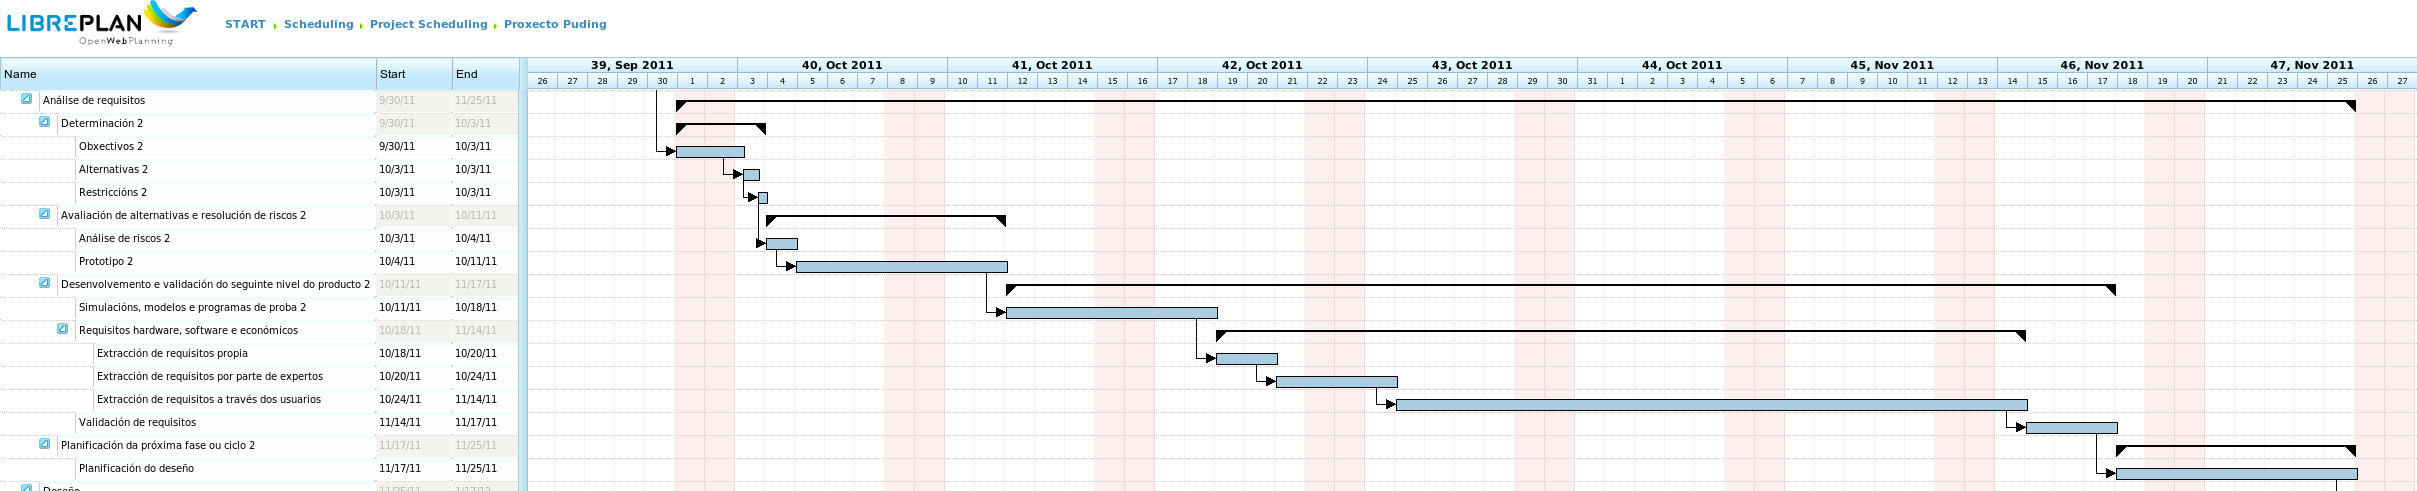
\includegraphics[scale=0.3,angle=90,keepaspectratio=true]{./imagenes/requisitos.png}
 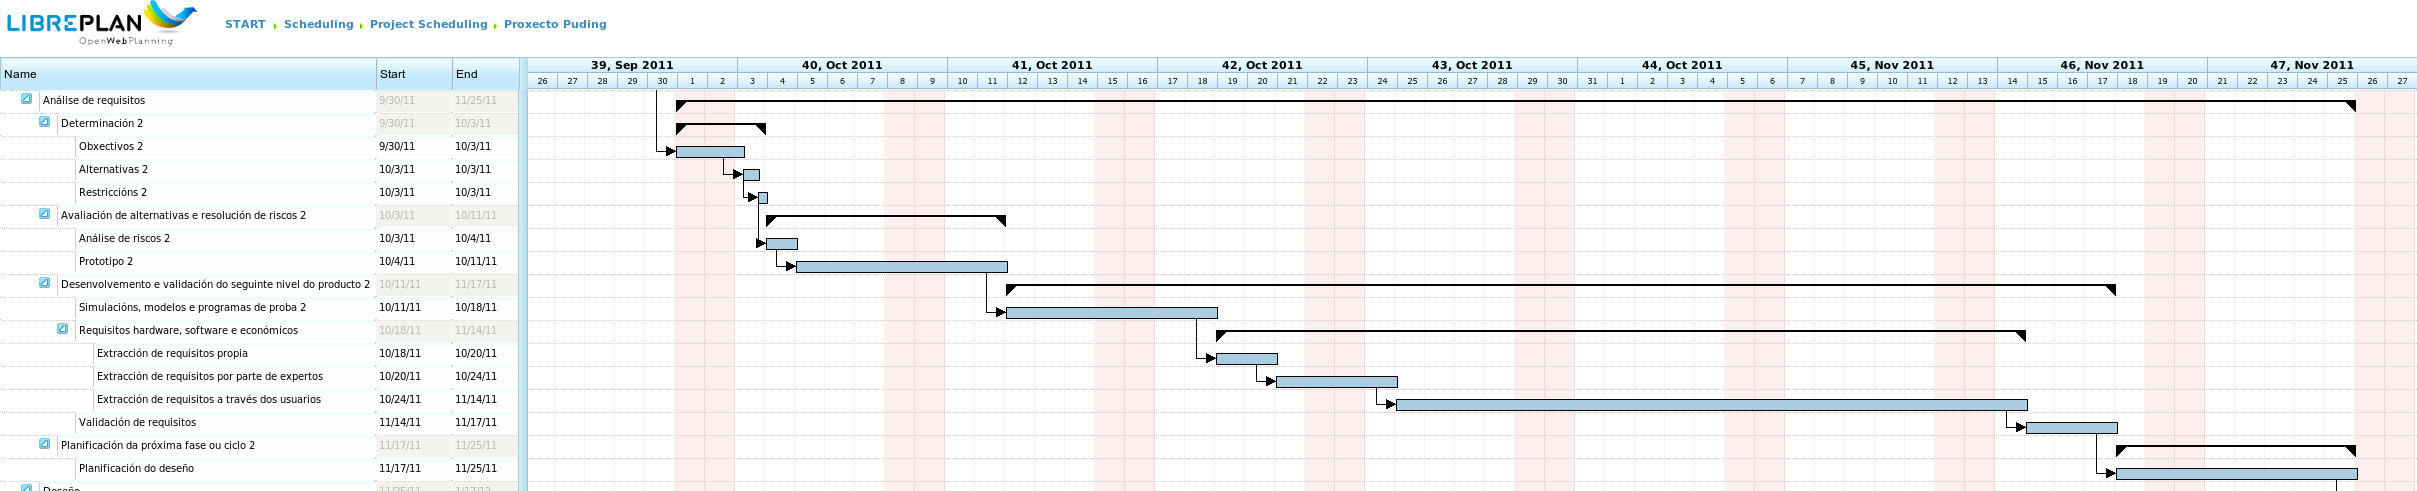
\includegraphics[trim=0 0 48cm 0,clip=true,scale=0.7,keepaspectratio=true]{./imagenes/requisitos.png}
 % requisitos.png: 2417x491 pixel, 100dpi, 61.39x12.47 cm, bb=0 0 1740 354
 \caption{Planificación inicial do ciclo de análise de requisitos.}
 \label{figura:PlanificacionInicialRequisitos}
\end{figure}

\textbf{Total:} 160 horas.

 \subsection{Planificación do ciclo de vida}

 A planificación do ciclo de vida expúxose xa no capítulo
 \ref{chap:planificacion} coa finalidade de dar unha visión global dos
 capítulos posteriores.

\section{Estudio de viabilidade}

A presente sección sitúase ó final do capítulo para non distorsionar a orde de
exposición das tarefas reflexadas na planificación.\\

Para estudio de viabilidade e a extracción de requisitos a través dos usuarios
creouse unha enquisa anónima dispoñible en liña \cite{Enquisa}. No presente
apartado centrarémonos exclusivamente na parte relacionada coa viabilidade do
proxecto. As relacionadas coa análise de requisitos comentaranse no capítulo
seguinte.\\

Na enquisa preguntábase sobre datos persoais non identificativos (idade,
procedencia), o seu perfil coma gaiteiro, coñecementos sobre as gaitas MIDI,
caracterísiticas (fixadas de antemán en extraccións previas) preferibles dunha
gaita MIDI e a súa prioridade, características propias a engadir e a súa
prioridade e un pequeno estudio económico.\\

A redacción da enquisa foi a seguinte:

\begin{quotation}
\itshape

 O Proxecto Puding trata de crear unha gaita MIDI integramente libre e galega.\\

 Esta enquisa está orientada a recoller or requisitos desexables dunha gaita
 MIDI e a estudiar o perfil do tipo de gaiteiro interesado nela.\\

 A enquisa é totalmente anónima (a excepción dos datos xeográficos e de idade)
 precisos para a elaboración do perfil. Tódolos datos recabados serán
 empregados exclusivamente para a fin anteriormente exposta.\\

 Os únicos requisitos desexables para cubrir esta enquisa son:

 \begin{itemize}
  \item Ser gaiteiro.
  \item Responder o máis completa e correctamente a mesma. Os datos
        incorrectos, incongruentes ou incompletos son contraproducentes para o
        estudio, polo que serán excluidos dos resultados.
 \end{itemize}

 Gracias de antemán.\\

 Enquisa:

 \begin{enumerate}
  \item ¿Que anos tes?
  \item ¿En que localidade resides?
  \item ¿A que provincia pertence dita localidade?
        \begin{enumerate}
         \item A Coruña.
         \item Lugo.
         \item Ourense.
         \item Pontevedra.
         \item Outra. ¿Cal?
        \end{enumerate}
  \item Como gaiteiro, ¿en que nivel te incluirías?
        \begin{enumerate}
         \item Principiante.
         \item Intermedio.
         \item Profesional.
        \end{enumerate}
  \item ¿Contas con gaita de teu?
        \begin{enumerate}
         \item Si.
         \item Non, só cun punteiro de iniciación.
         \item Non, pero téñoa encargada xa.
         \item Non.
        \end{enumerate}
  \item ¿Que pensas da aplicación da tecnoloxía actual ó mundo da gaita?
        \begin{enumerate}
         \item Creo que non aportaría vantaxes sobre o que hai.
         \item A tecnoloxía podería traer vantaxes, pero por tradición
               preferiría seguir empregando a gaita de toda a vida.
         \item Gustaríame preservar a maior parte da gaita tradicional, pero
               melloraría con tecnoloxía certos aspectos.
         \item A tecnoloxía está totalmente infrautilizada no mundo da gaita.
               Vai sendo hora de crear unha gaita 2.0.
        \end{enumerate}
  \item ¿Sabes o que é unha gaita ou punteiro MIDI?
        \begin{enumerate}
         \item Si.
         \item Non, pero teño escoitado falar delas.
         \item Non.
        \end{enumerate}
  \item En caso afirmativo, ¿coñeces algunha das seguintes?
        \begin{enumerate}
         \item Master Gaita
         \item Technopipe
         \item E-pipe
         \item Hevia Electronic Bagpipe
         \item Outra. ¿Cal?
        \end{enumerate}
  \item ¿Estarías interesado nunha gaita ou punteiro MIDI?
        \begin{enumerate}
         \item Si, teño pensado mercar unha.
         \item Si, pero só se cumpre coas miñas expectativas.
         \item Non, pero podería chegar a interesarme se xurde algo xeitoso.
         \item Non, de ningunha maneira.
        \end{enumerate}
  \item En caso afirmativo, ¿que uso lle darías? [Resposta múltiple]
        \begin{enumerate}
         \item Para ensaiar na casa.
         \item Para compoñer ou pasar pezas a un ordenador.
         \item Para empregar nas clases.
         \item Para empregar en concertos.
         \item Outro. ¿Cal?
        \end{enumerate}
  \item ¿Cales das seguintes características che gustaría que tivese? ¿Con que
        prioridade (1 a 5 -a maior número, maior prioridade-)?
        \begin{enumerate}
         \item Ausencia de retardos.
         \item Salvagarda da configuración entre usos.
         \item Presión regulable.
         \item Sensores dos dedos regulables independentemente.
         \item Afinación base regulable.
         \item Afinación regulable por nota.
         \item Dixitación personalizable.
         \item Sensor da presión do fol deshabilitable.
         \item Vibrato.
         \item Glisandos.
         \item Bordóns.
         \item Samples de calidade.
         \item Punteiro con forma tradicional.
         \item Punteiro acoplable a un fol calquera.
         \item Posibilidade de conexión a un ordenador.
         \item Conexión sen fíos.
        \end{enumerate}
  \item Indica outras características que che gustaría que tivese, ordeadas por
        prioridade.
  \item ¿Estarías disposto a mercar unha gaita MIDI coas características
        anteriores (incluidas as que ti mesmo engadiches)?
        \begin{enumerate}
         \item Si.
         \item Non.
        \end{enumerate}
  \item De ser así, ¿canto estarías disposto a pagar por unha?
  \item En caso contrario, ¿por que non?
  \item Sabendo que as gaitas MIDI presentes hoxe en día no mercado oscilan
        entre os 275 euros e os 2800 euros e que a maior parte delas non
        satisfacen as caracterísiticas anteriores ¿canto estarías disposto a
        pagar por unha que as incluíse todas ou case todas?
 \end{enumerate}
\end{quotation}

É de facer notar que as respostas a dita enquisa non son públicas, polo que
ningún usuario previo pode influir coas súas respostas sobre usuarios
posteriores. Evidentemente, esta medida está enfocada a evitar un posible
problema de falsa correlación forte nas respostas, o que podería invalidar
totalmente a enquisa.\\

Os resultados completos poden consultarse no apéndice \ref{chap:encuesta}.\\

Os resultados relativos á viabilidade foron os das seguintes figuras
(\ref{figura:ResultadosEstudioViabilidade1} a
\ref{figura:ResultadosEstudioViabilidade3}).\\

\begin{figure}[htbp]
 \centering
 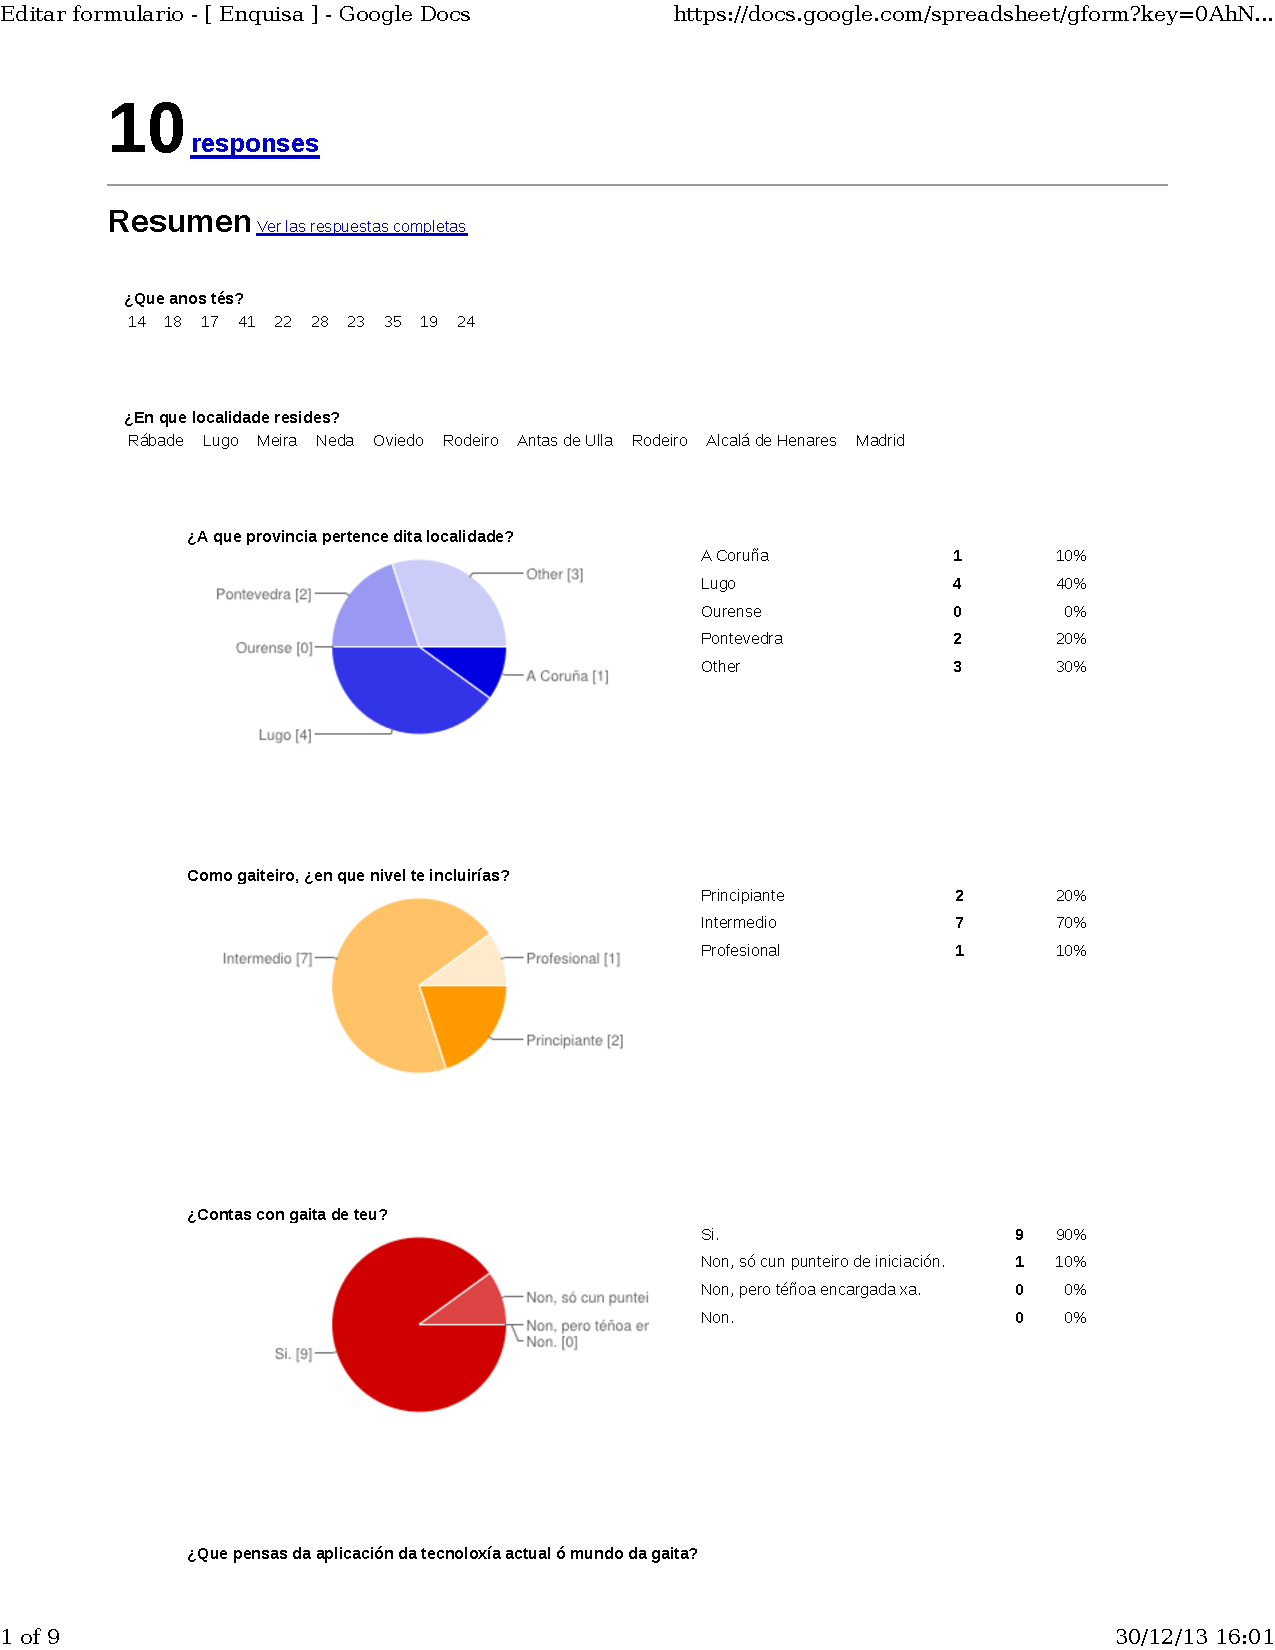
\includegraphics[scale=0.7,page=1,keepaspectratio=true,clip,trim=0cm 0.5cm 0cm 0.5cm]{./imagenes/enquisa.pdf}
 % enquisa.pdf: 612x792 pixel, 72dpi, 21.59x27.94 cm, bb=0 0 612 792
 \caption{Resultados do estudio de viabilidade (p. 1).}
 \label{figura:ResultadosEstudioViabilidade1}
\end{figure}

\begin{figure}[htbp]
 \centering
 \includegraphics[scale=0.7,page=2,keepaspectratio=true,clip,trim=0cm 0.5cm 0cm 0.5cm]{./imagenes/enquisa.pdf}
 % enquisa.pdf: 612x792 pixel, 72dpi, 21.59x27.94 cm, bb=0 0 612 792
 \caption{Resultados do estudio de viabilidade (p. 2).}
 \label{figura:ResultadosEstudioViabilidade2}
\end{figure}

\begin{figure}[htbp]
 \centering
 \includegraphics[scale=0.7,page=3,keepaspectratio=true,clip,trim=0cm 22cm 0cm 0.5cm]{./imagenes/enquisa.pdf}
 % enquisa.pdf: 612x792 pixel, 72dpi, 21.59x27.94 cm, bb=0 0 612 792
 \caption{Resultados do estudio de viabilidade (p. 3).}
 \label{figura:ResultadosEstudioViabilidade3}
\end{figure}

Tendo en conta estes resultados, podemos afirmar que o perfil xeral do gaiteiro
que respondeu a enquisa é o seguinte:

\begin{itemize}
 \item Menor de 30 anos.
 \item Galego e maiormente da provincia de Lugo.
 \item Con residencia fóra das capitais de provincia.
 \item Cun nivel intermedio coma gaiteiro.
 \item Con gaita de seu.
 \item Que lle gustaría preservar a maior parte da gaita tradicional, pero
       melloraría con tecnoloxía certos aspectos. Aínda que hai unha parte
       importante que aínda pensando que a tecnoloxía podería traer vantaxes,
       preferiría seguir empregando a gaita de toda a vida.
 \item Que coñece o concepto de gaita MIDI.
 \item Que coñece un ou varios modelos de gaitas MIDI existentes no mercado.
       Pero que curiosamente o máis vendido actualmente (e con moita
       diferencia) é o menos coñecido de todos.
 \item Que está interesado en mercar unha gaita MIDI se cumpre coas súas
       expectativas ou que podería chegar a estalo se xorde algo xeitoso.
\end{itemize}

Así mesmo, logo de respostar á parte referida ós requisitos (que como xa se
comentou, se exporá no seguinte capítulo), volvéuselles preguntar se estarían
dispostos a mercar unha gaita MIDI coas características expostas, incluíndo as
que eles mesmos reclamaban.

\begin{figure}[htbp]
 \centering
 \includegraphics[trim=0 12cm 0 11cm,clip=true,scale=0.7,page=8,keepaspectratio=true]{./imagenes/enquisa.pdf}
 % enquisa.pdf: 612x792 pixel, 72dpi, 21.59x27.94 cm, bb=0 0 612 792
 \caption{Resultados do estudio de viabilidade (p. 8).}
 \label{figura:ResultadosEstudioViabilidade8}
\end{figure}

Como se pode observar na figura \ref{figura:ResultadosEstudioViabilidade8}, a
resposta foi totalmente afirmativa, incluso por parte de aqueles que albergaban
dúbidas ó respecto, o que fai pensar que se vai por bo camiño. Por este motivo,
a pregunta sobre as razóns para non mercala quedou sen resposta. \\

A modo de avaliación da enquisa, comentar que é evidente que o número de
persoas que respostaron a enquisa é claramente non significativo. Se se aplica
o \textbf{problema de Fermi} \cite{ProblemaFermi} a este caso cos seguintes
datos:

\begin{itemize}
 \item Adoita haber 1 grupo de gaitas en cada concello.
 \item Cada grupo adoita estar composto por 10 músicos, dos cales a metade
       adoitan ser gaiteiros.
 \item Galicia conta con 315 concellos.
\end{itemize}

Pódese estimar entón que só en Galicia hai xa preto de 1600 gaiteiros. \\

Se se repite dita estimación co total de grupos rexistrados (273) na
\textit{Asociación de Gaiteiros Galegos} \cite{AGG} en lugar de concellos,
arroxa un total aproximado de 1400 gaiteiros. \\

Tomando como dato final a media de ditas estimacións, saen
\textbf{1500 gaiteiros}. \\

Polo que a mostra que se obtivo sería inferior ó 1\% do total estimado. Para que
a enquisa resultase significativa a mostra debería de ser bastante maior.\\

Supoñendo unha distribución normal e aplicando a fórmula para o cálculo do
tamaño mostral coñecido o tamaño da poboación \cite{TamanoMuestra}:

\begin{equation}
 n = \frac{N}{1 + \frac{e^2(N-1)}{(z^2)pq}}
\end{equation}

Onde:

\begin{itemize}
 \item \textit{n}, é o tamaño da mostra.
 \item \textit{N}, o tamaño da poboación.
 \item \textit{e}, o erro mostral (marxe de erro admitida).
 \item \textit{z}, valor de \textit{z} correspondente ó valor de confianza.
 \item \textit{pq}, a varianza da poboación; onde se $p = q = 0.5$ (a metade
       dos suxeitos responde afirmativamente e a outra negativamente), entón
       $pq = 0.25$ (cte.).
\end{itemize}

Para valores:

\begin{itemize}
 \item Nivel de confianza do 95\%.
 \item $N = 1500$.
 \item $e = 0.1$.
 \item $z = 1.96$ ($\alpha = 0.05$).
 \item $pq = 0.25$.
\end{itemize}

Entón:

\begin{equation}
 n = \frac{1500}{1 + \frac{0.1^2(1500-1)}{(1.96^2)0.25}} \approx 90
\end{equation}

É dicir, precisariamos que uns 90 gaiteiros (un 6\% da poboación) respondesen á
enquisa. \\

Aínda tendo en conta o anterior, tendo evitado o condicionamento entre usuarios
e vista a dispersión mostral, os resultados da enquisa parecen amosar unha
forte correlación verdadeira, motivo polo cal tendemos a crer que o proxecto é
comercialmente viable desde o punto de vista de interés do mercado no producto.
